
\documentclass[a4paper,12pt]{article} % тип документа


% Русский язык
\usepackage[T2A]{fontenc} % кодировка
\usepackage[utf8]{inputenc} % кодировка исходного текста
\usepackage[russian,english]{babel} % локализация и переносы
\usepackage{graphicx}
\graphicspath{{pictures/}}
\DeclareGraphicsExtensions{.pdf,.png,.jpg}


% Математика
\usepackage{amsmath,amsfonts,amssymb,amsthm,mathtools}


\usepackage{wasysym}

%Заговолок
\author{Талашкевич Даниил Александрович}

\title{Лабораторная работа 1.1.6}

\date{\today}

\begin{document}

\maketitle
\thispagestyle{empty}

\newpage
\setcounter{page}{1}


{\bf 1. Аннотация }\\ Ознакомиться с устройством и работой осциллографа, изучить его основные харак-
теристики. Измерить амплитудно-частотные характеристики (АЧХ) усилителей каналов  $"X"$ и  $"Y"$ ,а также измерить их фазово-частотную разность.\\
{\bf 2. Теоретические сведения }

\hspace{1mm} 1.Устройство ЭЛТ осциллографа:
\begin{center}
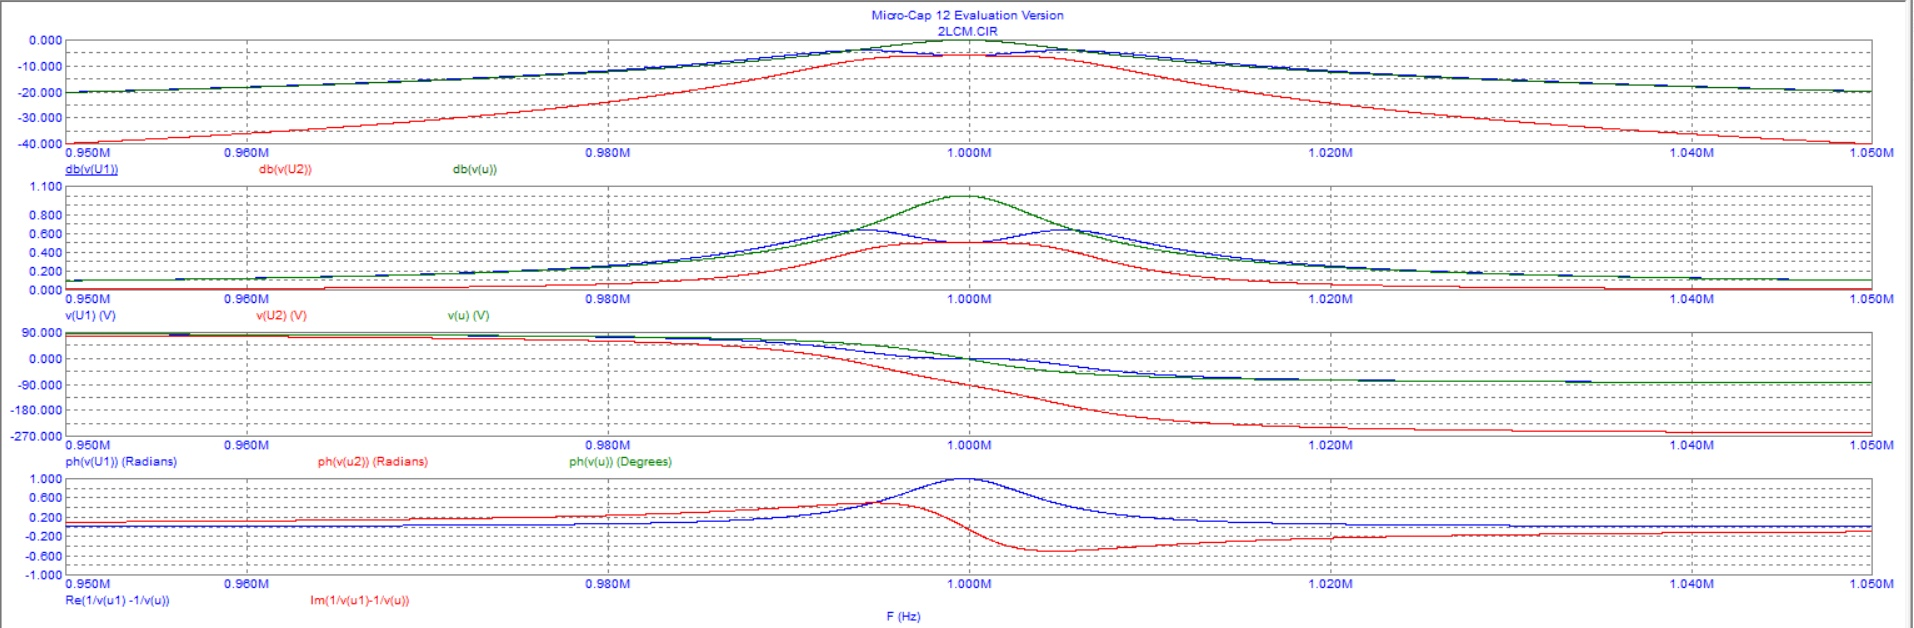
\includegraphics[width=\textwidth]{1.1.6}
\end{center}
Рис. 1: Где 1-подогреватель катода, 2- катод, 3-модулятор, 4- первый (фокусирующий)
анод, 5- второй (ускоряющий ) анод, 6 и 7- горизонтально и вертикально отклоняющие
пластины, 8- третий (ускоряющий) анод, 9- экран.\\
{\bf 2.1. Теория }\\
\hspace{2mm}1. Смещение $h$ электронного пятна на экране осциллографа: ${\bf h =\frac{l_1L}{2dU_\alpha}\cdot U_y.}$\\
Чувствительность трубки к напряжению: ${\bf k =\frac{l_1L}{2dU_\alpha}}$, где ${\bf l_1}$ -- длинна пластин, ${\bf L}$ - расстояние от середины пластин до экрана, $d$ -- расстояние между пластинами,$\bf{ U_\alpha} $ -- ускоряющее напряжение на втором аноде.\\
\hspace{2mm}2.Подаваемое на вертикально отклоняющие пластины напряжение должно быть пропорционально самому сигналу:  ${\bf U_y(t) = U_{0y}+K_{yu}U_c(t).}$\\
${\bf U_{0y}}$ -- постоянное напряжение, определяющие расположение графика сигнала по оси $Y$ ; ${\bf K_{uy}}$ -- коэффициент входного сигнала каналом вертикального отклонения.\\
Подаваемое на горизонтально отклоняющие пластины напряжение должно линейно зависить от времени : ${\bf U_x = U_{0x}+ K_{xu}t}$, где ${\bf U_{0x}}$ -- постоянное напряжение, определяющие расположение графика сигнала по оси $Х$ ; ${\bf k_{xu}}$ -- коэффициент пропорциональности, зависящий от рабочих харрактеристик генератора развертки и усилителя.\\
Отношение максимальной и минимальной амплитуд генератора: ${\bf \beta [\textbf{дБ}] = 20\ lg(\frac{A}{A_0})}$.\\
Коэффициент ослабления сигнала К: ${\bf K(f_{\textbf{эг}}) = \frac{2A(f_{\textbf{эг})}}{2A_0}}$.\\
\hspace{2mm}3. Фигуры Лиссажу Напряжение на горизонтально отклоняющие пластины: ${\bf U_x = U_\alpha \cos (2\pi ft + \varphi_{1})}$.\\
Напряжение на вертикально отклоняющие пластины: ${\bf U_x = U_b \cos(2\pi ft + \varphi_{2})}$.\\
Тогда уравнение траектории движении луча: ${\bf \frac{x^2}{A^2}+\frac{y^2}{B^2}+2\frac{xy}{AB}\cos(\varphi_2 - \varphi_1)} = \sin^2(\varphi_2 - \varphi_1)$.\\
{\bf 3. Используемое оборудование: }\\
1) Осциллограф;\\
2) Генераторы электрических сигналов;\\
3) Соединительные кабели.\\
{\bf 4. Ход работы: }\\ \\
{\bf 4.1 Наблюдение периодического сигнала от генератора и измере-
ние его частоты.}\\
Предварительно выполнив все иструкции, прописанные в руководстве, получим устойчивое изоб-
ражение и настроим мастштаб так, чтобы изображение занимала как можно больше места на экране.\\
В таблице ниже приведены результаты измерений периода сигнала от подаваемой частоты по формуле ${\bf f =\frac{1}{T}}$.\\
По данным значениям построим график ${\bf K_{AC}(lg\ f)}$ и ${\bf   K_{DC}()lg f}$.\\
Однако, как видно из таблицы, значения ${\bf U_{DC}}$ и ${\bf U_{AC}}$ совпадают во всех точках, поэтому это будет
один и тот же график.\\
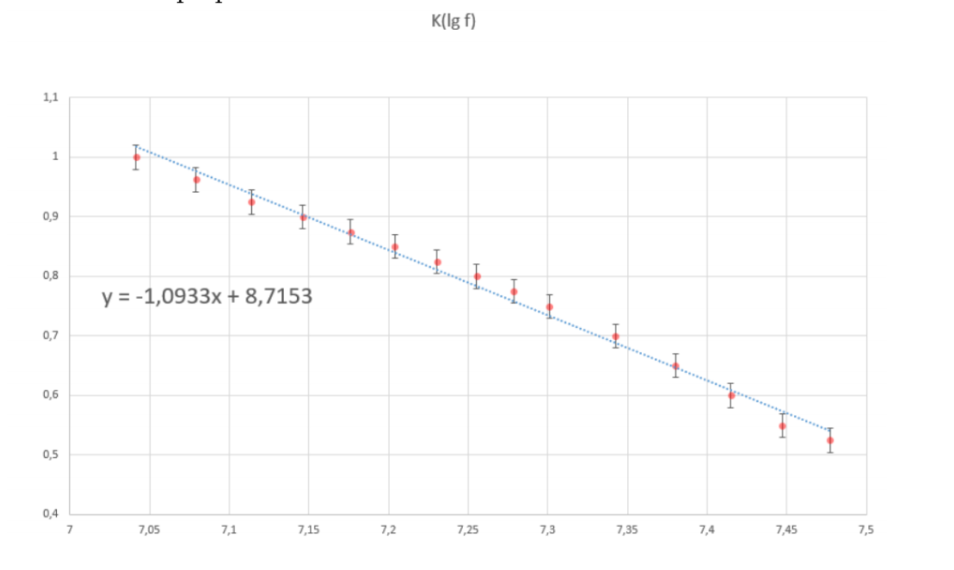
\includegraphics[width=\textwidth]{1.1.6 1}
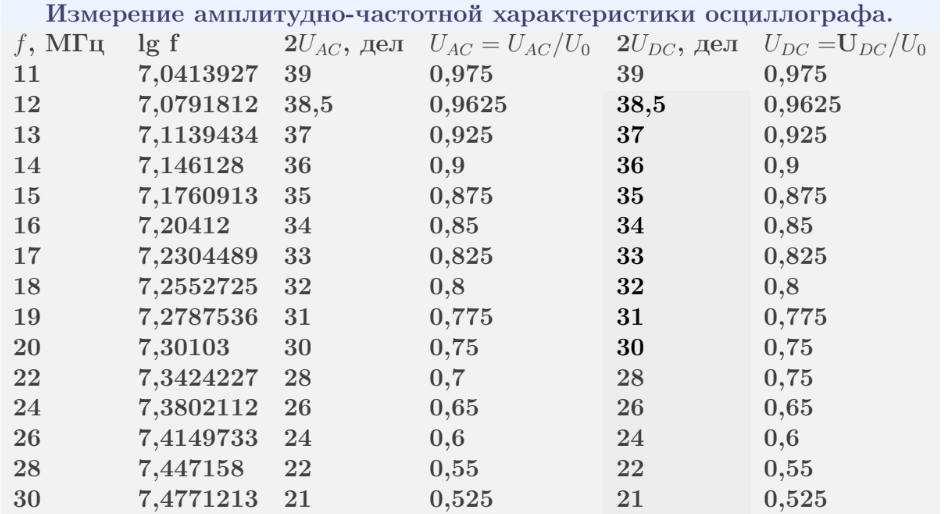
\includegraphics[width=\textwidth]{1.1.6 2}\\
Как можно видеть, значение ${\bf K(f) = \frac{U(f)}{U_0}}$ линейно спадает с ростом ${\bf lg(f)}$, а значит, и частоты входящего сигнала. Такое резкое понижение начинается при ${\bf f \approx 10\textbf{МГц}}$.\\
Погрешность ${\bf \sigma_\textbf{K}}$ можно рассчитать как: ${\bf  \sigma_\textbf{K} = \sqrt{(\frac{\bigtriangleup U}{U})^2 + (\frac{\bigtriangleup U_0}{U_0})^2}}$.Возьмем максимльное значение ${\bf U}$, тогда ${\bf \sigma_\textbf{K} = 0,0345.}$\\
Из гафика получаем, что коэффициент наклона ${\bf k}$ аппроксимирующей прямой, построенной с помощью метода наименьших квадратов, приблизительно равен ${\bf - 1.09}$. Получим формулу для учета погрешности измерения амплитуды на высоких частотах:\\
\[ U^{'} = U + 1.09\cdot U  |lg f - 7.15| .\]\\
где ${\bf U^{'}}$ -- настоящее значение амплитуды, ${\bf U}$ -- измеренная амплитуда.

{\bf 4.2 Измерение разности фазово-частотных характеристик каналов осциллографа}\\
Для изученя ФЧХ осциллографа подадим сигнал на каналы X и Y. Будем менять значения фаз для получения элипса, задаваемого формулами:\\${\bf x(t) = A_x\sin(\omega t + \phi_x)}$, ${\bf y(t) = A_y \sin(\omega t + \varphi_y)}$.\\
Пусть ${\bf \omega t = - \phi_x}$. Тогда ${\bf \sin(|	\bigtriangleup \phi|) = |\frac{y_0}{A_y}|}$, где ${\bf y_0}$ -- отклонение по вертикали в момент ${\bf х=0}$.\\
Используя метод показанный ниже, заполним таблицу и получим зависимость ${\bf \bigtriangleup \phi (lg f)}$.\\

\includegraphics[width=\textwidth]{1.1.6 3}\\
Построим графики зависимости ${\bf \bigtriangleup \phi}$ от ${\bf lg f}$ и ${\bf f}$:\\
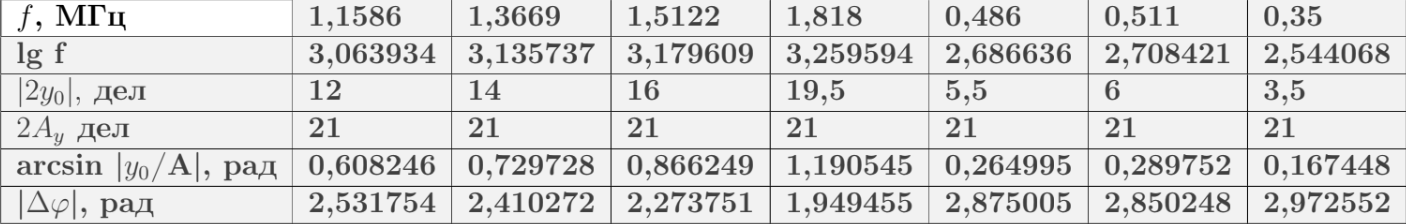
\includegraphics[width=\textwidth]{1.1.6 4}\\
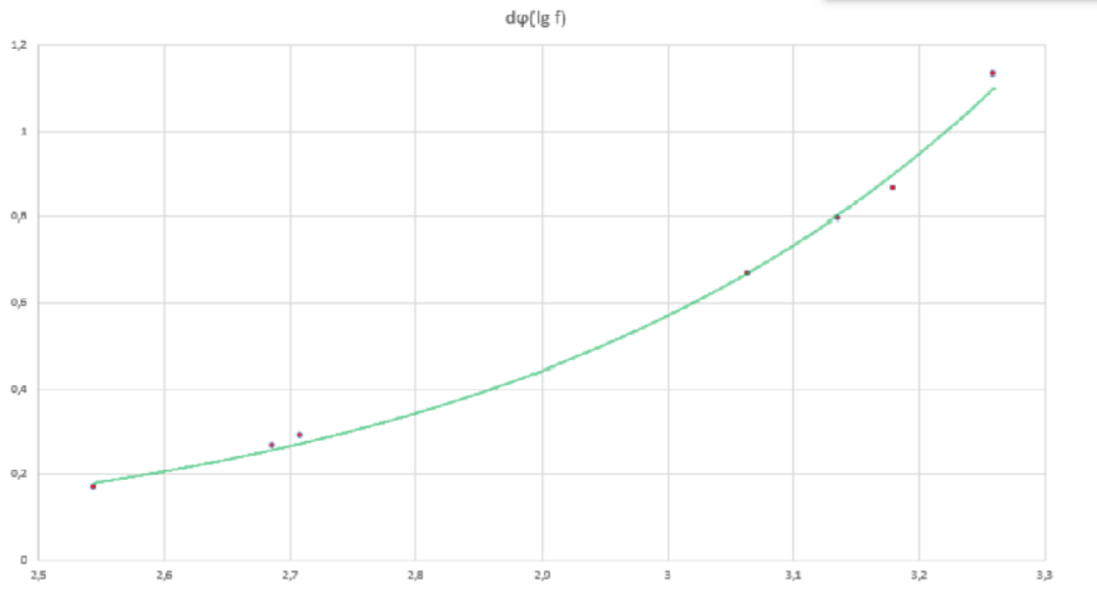
\includegraphics[width=\textwidth]{1.1.6 5}\\
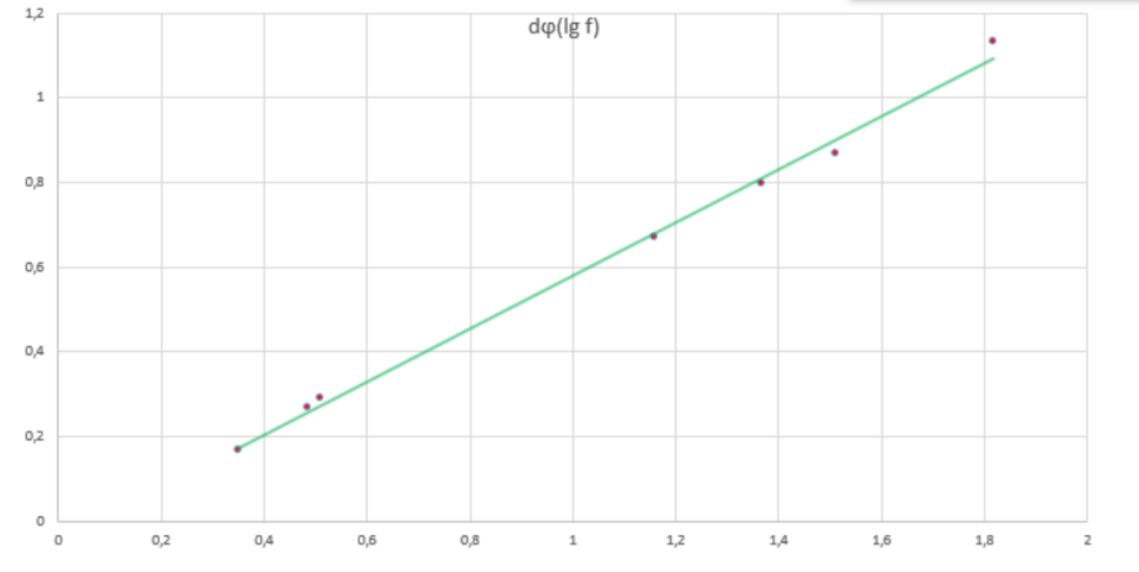
\includegraphics[width=\textwidth]{1.1.6 6}\\
Видно, что первая зависимость имеет экспоненциальный харрактер, а вторая линейный. Также можно заметить, что с возрастанием частоты отклонение точке от аппроксимирующей прямой,слудовательно осциллограф может быть использован для определения разности фаз только при сравнительно небольших частотах.\\
{\bf 4.3 Наблюдение фигур Лиссажу }\\
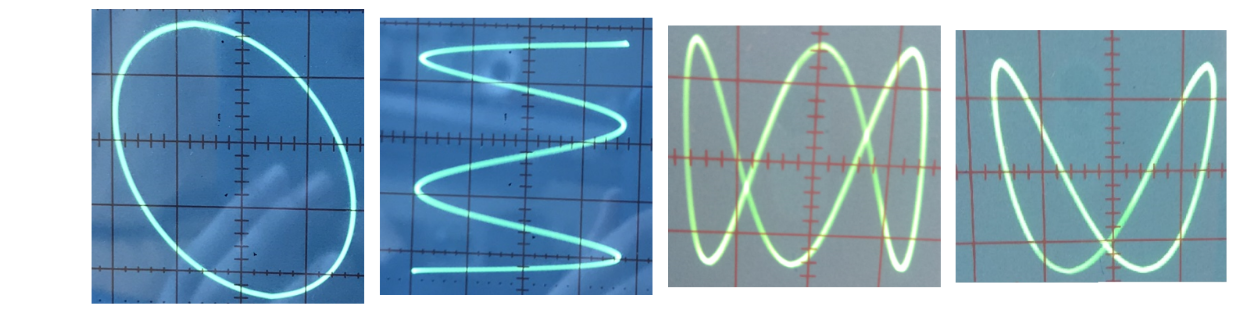
\includegraphics[width=\textwidth]{1.1.6 7}\\
{\bf 5 Вывод }\\
В данной работе мы познакомились с устройством и принципом работы осциллографа. Мы построили графики АЧХ и ФЧХ и выяснили, что на низких частотах осциллометр позволяет производить рассчеты с достаточно высокой точностью.






${\bf }$









\end{document}


